\section{Habib Abdul Rasyid}
\subsection{ Apa itu fungsi device manager di windows dan folder /dev di linux}
Device Manager adalah Panel Kontrol dalam sistem operasi Microsoft Windows. Ini memungkinkan pengguna untuk melihat dan mengontrol perangkat keras yang terpasang pada komputer. Ketika beberapa bagian perangkat keras tidak berfungsi, perangkat keras yang terkait akan disorot oleh pengguna. Daftar perangkat keras dapat disortir berdasarkan berbagai kriteria.
Untuk setiap perangkat, pengguna dapat:
\begin{itemize}
     \item Menyediakan driver perangkat sesuai dengan Model Driver Windows
     \item Aktifkan atau nonaktifkan perangkat
     \item Beri tahu Windows untuk mengabaikan perangkat yang tidak berfungsi
     \item Lihat sifat teknis lainnya
\end{itemize}
Device Manager diperkenalkan dengan Windows 95 dan kemudian ditambahkan ke Windows 2000. Dalam versi berbasis NT, ini dimasukkan sebagai snap-in Konsol Manajemen Microsoft.\newline

/ dev adalah lokasi file khusus atau perangkat. Ini adalah direktori yang sangat menarik yang menyoroti satu aspek penting dari sistem file Linux - semuanya adalah file atau direktori.


\subsection{Jelaskan langkah-langkah instalasi driver dari Arduino}
Berikut ini merupakan langkah-langkah untuk melakukan instalasi driver Arduino
\begin{itemize}
	\item Pertama-tama, pasang board arduino pada pc. Kemudian tunggu sampai windows mencoba menginstal sendiri. jika gagal, lanjutkan ke step selanjutnya
	\item buka Device Manager 
	\item Cari nama arduino atau "Unknown Device"
	\item klik kanan pada unknown device , dan pilih update software
	\item Cari folder instalan software arduino
	\item klik Next
	\item Jika telah berhasil, maka proses instal driver sudah selesai
\end{itemize}

\subsection{Jelaskan bagaimana cara membaca baudrate dan port dari komputer yang sudah terinstal driver}
Berikut ini merupakan cara membaca baudrate dan port dari komputer yang sudah terinstal driver :
\begin{itemize}
	\item Sambungkan port USB arduino dengan port USB pc
	\item Kemudian buka software arduino pada pc
	\item Setelah itu, pilih tipe arduino yang digunakan
	\item Kemudian memilih serial port yang aktif  
	\item Selanjutnya untuk memasukkan program pada arduino, klik tombol upload
	\item Setelah proses upload selesai, buka fitur serial monitor
	\item Lalu sesuaikan Baudrate pada serial monitor dengan Baudrate yang terdapat pada program
\end{itemize}

\subsection{Jelaskan sejarah library pyserial}
Pyserial berguna untuk merangkum akses untuk port serial. Pyserial menyediakan backends untuk Python yang berjalan di Windows, Linux, BSD (mungkin sistem yang mendukung POSIX), Jython dan IronPython (.NET dan Mono). Modul bernama "serial" secara otomatis memilih backend yang sesuai. Antarmuka berbasis kelas yang sama pada semua platform yang didukung.
Akses ke pengaturan port melalui properti Python.
Dukungan untuk berbagai ukuran byte, bit stop, paritas dan kontrol aliran dengan RTS / CTS dan / atau Xon / Xoff.
Bekerja dengan atau tanpa menerima batas waktu.
File seperti API dengan "read" dan "write" ("readline" dll. Juga didukung).
File-file dalam paket ini adalah 100 persen Python murni.
Port diatur untuk transmisi biner. Tidak ada stripping byte NULL, terjemahan CR-LF dll. (Yang berkali-kali diaktifkan untuk POSIX.) Ini membuat modul ini bermanfaat secara universal.
Kompatibel dengan pustaka io (Python 2.6+)

\subsection{Jelaskan fungsi-fungsi apa saja yang dipakai dari library pyserial}
Serial – fungsi ini untuk membuka port serial
Write(data) – untuk menulis data lewat port serial
Readline() – untuk membaca string dari port serial
Read(size) – untuk membaca jumlah byte dari port serial
Close() – ini untuk menutup port serial 

\subsection{Jelaskan kenapa butuh perulangan dalam tidak butuh perulangan dalam membaca serial}
Perualangan dalam bahasa pemrograman berfungsi menyuruh komputer melakukan sesuatu secara berulang-ulang. Terdapat dua jenis perualangan dalam bahasa pemrograman python, yaitu perulangan dengan for dan while.
Perulangan for disebut counted loop (perulangan yang terhitung), sementara perulangan while disebut uncounted loop (perulangan yang tak terhitung). Perbedaan yang terlihat adalah pada perulangan for digunakan untuk mengulangi kode yang sudah diketahui banyak perulangannya. Sedangkan perulangan while digunakan pada perulangan yang memiliki syarat dan tidak tentu berapa banyak perulangannya.
Perulangan diperlukan agar dapat membaca data secara berulang kali sehingga data yang muncul lebih dari satu.  Sedangkan apabila tidak memakai perulangan maka data akan terbaca satu kali saja.

\subsection{Jelaskan bagaimana cara membuat fungsi yang mengunakan pyserial}
Berikut merupakan contoh penggunaan fungsi yang menggunakan pyserial
\lstinputlisting[firstline=5, lastline=15]{src/5/Teori/T1174002.py}

\subsection{Plagiarisme}
\begin{figure}[h]
\centering
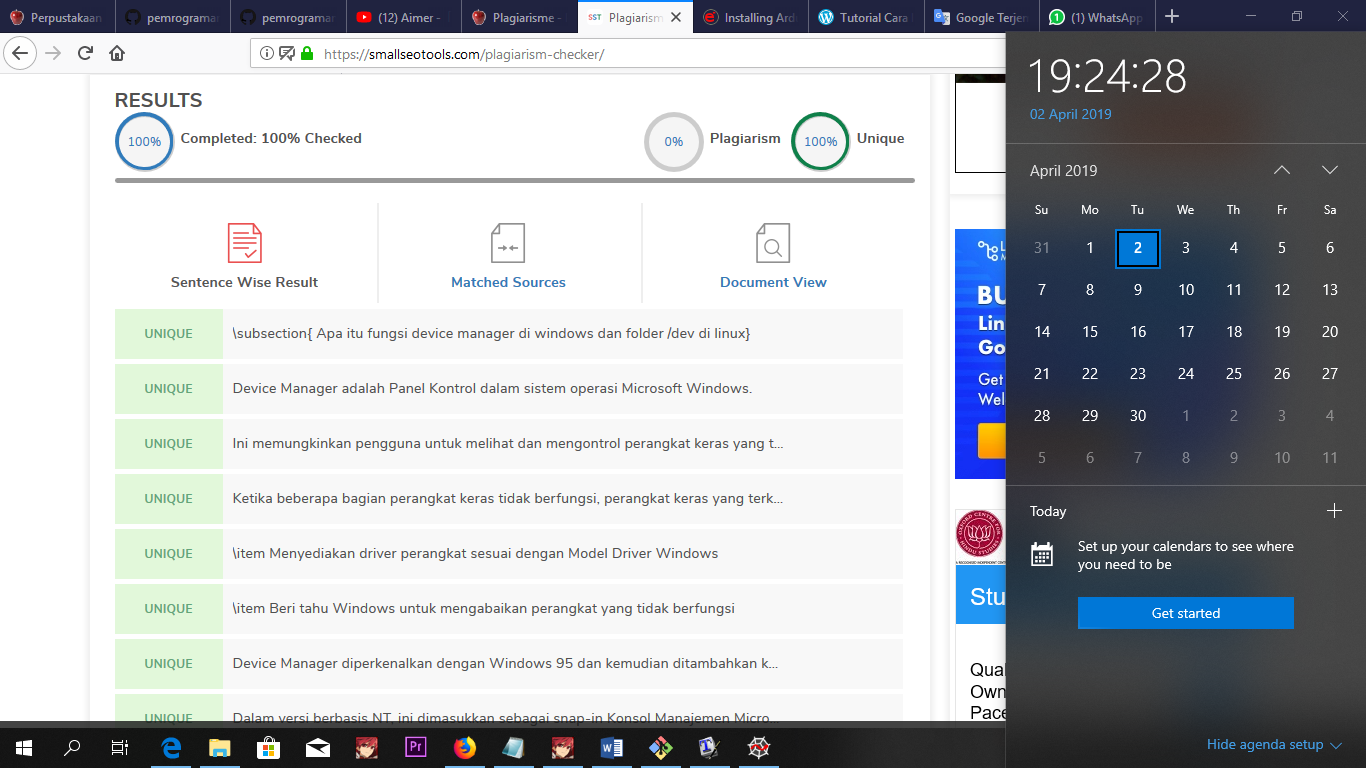
\includegraphics[scale=0.2]{figures/5/Teori/1174002/plagiat.png}
\caption{Plagiarisme}
\label{fig:plagiat}
\end{figure}

\section{Rahmatul Ridha}
\subsection{Soal 1}
Isi jawaban soal ke-1

Kalau mau dibikin paragrap \textbf{cukup enter aja}, tidak usah pakai \verb|par| dsb

%\subsection{Soal 2}
%Isi jawaban soal ke-2

%\subsection{Soal 3}
%Isi jawaban soal ke-3

\section{Tomy Prawoto}
\subsection{Soal 1}
Isi jawaban soal ke-1

Kalau mau dibikin paragrap \textbf{cukup enter aja}, tidak usah pakai \verb|par| dsb

%\subsection{Soal 2}
%Isi jawaban soal ke-2

%\subsection{Soal 3}
%Isi jawaban soal ke-3
